% Requires running Bibtex

\documentclass[%
reprint,
amsmath,amssymb,
aps,
]{revtex4-2}

\usepackage{graphicx}% Include figure files
\usepackage{dcolumn}% Align table columns on decimal point
\usepackage{bm}% bold math
\usepackage{hyperref}% add hypertext capabilities
\usepackage[font=scriptsize,labelfont=bf, justification=justified]{caption}% change fontsize in captions
\usepackage{float}
\usepackage{booktabs}% cool table style
\hypersetup{
	colorlinks=true,       % false: boxed links; true: colored links
	linkcolor=black,        % color of internal links
	citecolor=black,        % color of links to bibliography
	filecolor=black,     % color of file links
	urlcolor=black         
}

\usepackage{bibspacing}
\setlength{\bibitemsep}{.5\baselineskip plus .05\baselineskip minus .05\baselineskip}


\begin{document}
	
	\preprint{APS/123-QED}
	
	\title{PHYC30170 Physics with Astronomy and Space Science Lab 1;\\An Investigation of Surface Plasmon Resonance}
	
	\author{Daragh Hollman}
	\email{daragh.hollman@ucdconnect.ie}
	
	\date{\today}
	
	\begin{abstract}
		The aims of this experiment were to determine the excitation angle of surface plasmon resonance (SPR) using the Kretschmann configuration, and observe and investigate the dependencies it has on the wavelength of the incident light and the thickness of the silver film used. We found that the excitation angle of SPR has both an inverse dependence on the wavelength of the incident light and an inverse dependence on the thickness of the silver film.  At a film thickness of 13 nm we determined the excitation angle to be $(43.9\pm0.5)^\circ$, $(44.6\pm0.5)^\circ$, and $(50.0\pm0.5)^\circ$ for the 633 nm, 515 nm, and 405 nm laser respectively.
	\end{abstract}

	\maketitle
	
	\section{Introduction}		
		Surface plasmons are transverse magnetic waves, comprised of oscillating electrons, which travel along the boundary of a metal and a dielectric \cite{undergradToledo}. They were first discovered in 1957 by R. H. Ritchie. The study of surface plasmons is very important and has many applications in biophysics, particularly in the analysis of biomolecular interactions \cite{biomedicalApplications}, and in many fields of optics including but not limited to sub-wavelength optics and near-field optics \cite{opticalApplications}.
	
	\section{Theory}
		\subsection{Excitation of Free Electrons}
			The free electrons in the conduction band of metallic substances can be excited to oscillate with an eigenfrequency described by the plasma frequency \cite{pluchery}. The collective coherent oscillations of these electrons on the surface of a metallic substance give rise to a longitudinal charge density wave which is known as a surface plasmon polariton or surface plasmon wave \cite{pluchery}\cite{zeng}. One way to detect these waves is through the coupling of them with an electromagnetic field.
			
		
		\subsection{Surface Plasmon Waves}
			
			The surface plasmon wave is derived from the dispersion equations, the boundary conditions applied to the electric field, and the electric displacement \cite{pluchery}. The wave vector acting in the axis of propagation is written as:
			\begin{equation}
				k_x^2 = \frac{\omega^2}{c^2} \cdot \frac{\epsilon_1(\omega) \cdot \epsilon_2(\omega)}{\epsilon_1(\omega) + \epsilon_2(\omega)}
				\label{eq:spWave}
			\end{equation}where $\omega$ is the angular frequency and $\epsilon(\omega)$ the dielectric function where the subscripts represent the respective media of the metal and the air. It is only necessary to discuss the effect in this axis as the plasmons are confined to the plane of the silver film and so for surface plasmon resonance, only the vector component parallel to the surface is important \cite{sprTheory}.\\
		
			When total internal reflection occurs the incident light reflecting off the film create an electric field on the opposite side of the interface. This field is called an evanescent wave as its amplitude decreases exponentially with increasing distance from the surface of the interface \cite{sprTheory}. This evanescent wave on the interface of the prism and silver has a dispersion relation dependent on the angle of incidence:
			\begin{equation}
				\omega = \frac{k_x \cdot c}{n \cdot \sin{\theta_\text{int}}}
				\label{eq:omega}
			\end{equation}where $n$ is the refractive index of the prism and $\theta_\text{int}$ is the internal angle of incidence marked in figure \ref{fig:angles}. This excites the surface plasmons and the condition for the coupling of the excitation wave and the surface plasmon wave is therefore given by combining equations \ref{eq:spWave} and \ref{eq:omega} \cite{pluchery}:
			\begin{equation}
				\left(n \, \sin{\theta_\text{int}}\right)^2 = \frac{\epsilon_1(\omega) \cdot \epsilon_2(\omega)}{\epsilon_1(\omega) + \epsilon_2(\omega)}
				\label{eq:combination}
			\end{equation}Note as we are dealing with the interface of silver and air, $\epsilon_2=1$, and because of this equation \ref{eq:combination} can then be reduced to an expression for the internal angle.\\
			\begin{equation}
				\theta_\text{int} = \arcsin\left(\frac{1}{n} \sqrt{\frac{\epsilon_1(\omega)}{\epsilon_1(\omega) + 1}}\right)
				\label{eq:angle}
			\end{equation}
			
			Therefore by using this equation to calculate the expected angle of incidence which will excite surface plasmon resonance, we can then compare this to what values are measured.
		
			\begin{figure}
				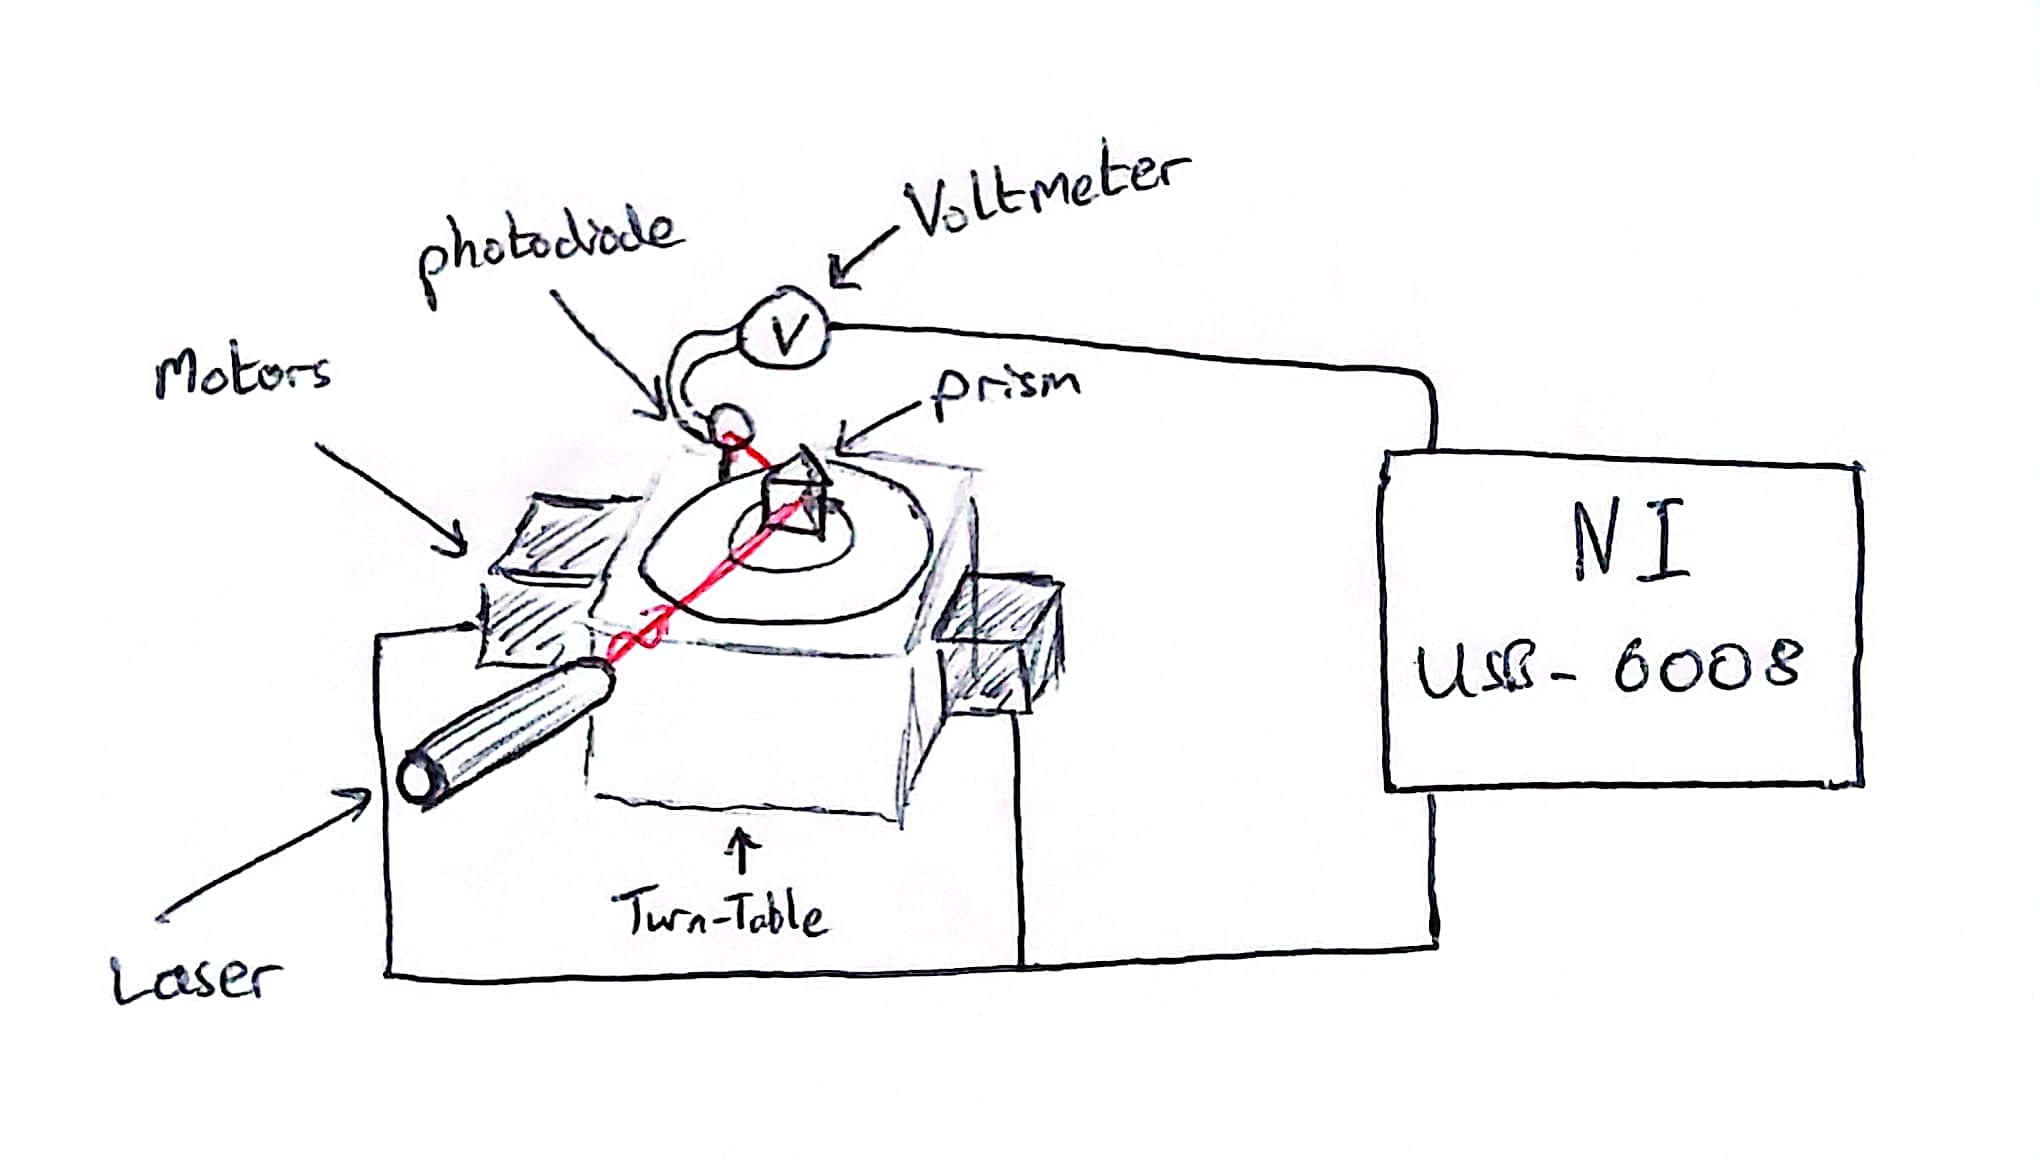
\includegraphics[width=0.85\columnwidth]{SPdiagram.jpg}
				\caption{\label{fig:apparatus}A diagram of the apparatus used. A laser shines through a polarising filter (not pictured) and intro a prism where it reflects off a thin silver film on the opposite side of the prism. The reflected light is detected by a photodiode and a voltmeter. The motors are controlled by a separate motor controller device which is not pictured. The NI USB-6008 device was connected to a computer to control the apparatus.}
			\end{figure}
			\begin{figure}
				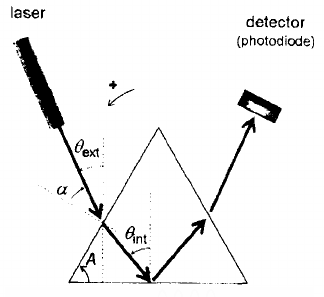
\includegraphics[width=0.7\columnwidth]{anglesDiagram.png}
				\caption{\label{fig:angles}The Kretschmann configuration. The silver film was evaporated onto the glass prism. The light from the laser excites the electrons and a surface plasmon polariton is formed on the outer side of the film. The diagram includes the external and internal angles \cite{pluchery}. Although an equilateral triangular face is shown, a prism with angles of $90^\circ$ and $45^\circ$ was used in this experiment.}
			\end{figure}
	 
	\section{Methodology}
		\subsection{Apparatus Setup}
			The apparatus was set up in the Kretschmann configuration as shown in figure \ref{fig:angles}. As only the external angle $\theta_\text{ext}$ could be directly measured, a simple equation was used to convert to the the internal angle $\theta_\text{int} \cite{pluchery}$.
			\begin{equation}
				\theta_\text{int} = \arcsin{\left( \frac{\sin{\left(\theta_\text{ext}-A\right)}}{n} \right)} + A
			\end{equation}where $n$ is the refractive index and $A$ is the angle of inclination of the prism, in our case $45^\circ$. \\
		
			The silver film was evaporated onto three prisms so that the thickness of the film could be varied. Thicknesses of 10nm, 13nm, and 15nm were used. The prism was placed in the centre of a bidirectional stepping rotary table. This table had two independently movable discs (specifically one disc and one annulus) controlled by stepper motors which, through a gear system, had a precision calibrated to be $0.045$ degrees per step. The prism was placed on the inner disc and a photodiode was fixed on the outer annulus to be used as a detector.\\
			
			The apparatus was controlled using Python 3 to interface with a USB multifunction I/O device, NI USB-6009 \cite{nationalInstruments}. This was used as a digital to analogue converter to control the stepper motors as well as an input from the photodiode to read voltages. A laser was placed into a retort stand such that it would pass through the prism and reflect off the silver film into the photodiode.

			\subsubsection{Light Source}
				Three He-Ne lasers were used of wavelengths 633nm, 515nm, and 405nm all of which had a maximum power $\le 4 \,\text{mW}$. In this report we will refer to these lasers as red, green, and blue respectively. A linear polarising filter was positioned between the laser and the prism such to p-polarise the incident light.
			
			\subsubsection{Motor Programming and an Algorithm for Data Collection}
				The stepper motor modules were programmed following the documentation provided by UCD Advanced Physics Labs \cite{motorDoc}. They were controlled by digital signals to the control lines of the USB I/O device. The control lines were used to enable and disable the motors, set the direction, and to advance each motor. We initially had issues getting these inputs to work as one of the pins was wired in contrast to the documentation, however through exhaustive testing we were able to identify the correct pins for each input. A function was then written in Python to control the movement of these motors. This function took inputs of a number of steps, a direction, and a delay time. It was important to include a short delay ($\approx 100\,\text{ms}$) between steps to reduce unwanted vibrational artefacts in the data and to not overheat the motors during extended use. Functionality was also included to select to rotate either the prism, or the detector, or both. This function is included in appendix A.1 on data acquisition. Note that the detector had to move twice for every prism step to keep the laser tracked on the detector due to their separation.\\
			
				This function was then edited to add capabilities to include data collection from the photodiode while moving. After each step 100 samples of the voltage were taken at $10,000\,\text{Hz}$. The mean of these was recorded as the voltage value and the standard deviation was taken as the uncertainty. To improve efficiency, functionality to drive the system backwards as well as forwards was introduced to remove the time taken to reset the apparatus to its initial position.\\

			\subsubsection{Laser Alignment}
				The laser, detector, and prism were aligned such that the right angled side of the prism was facing towards the laser and the beam was reflected back towards itself. We define this as an external angle of $0^\circ$. This was then moved $30^\circ$ degrees clockwise and the detector was moved into the path of the reflected beam.
			
		\subsection{Data Collection}
			To take data, the apparatus was set to an initial angle of approximately $30^\circ$. The data function was executed and the prism and the detector slowly rotated. Care was taken to ensure that the laser stayed tracked on the centre of the photodiode as if there were any misalignments it would drift off and the data would be inaccurate. The code ran for $600$ steps equivalent to an angular distance of $27^\circ$. The mean voltages across each step of this arc were recorded along with their standard deviations. This was done several times to improve accuracy and then repeated for all three lasers before switching to a $13\,\text{nm}$ prism and then repeated again for a $15\,\text{nm}$ prism. Note that an initial angle of $43.65^\circ$ was used for the blue laser as its excitation angle was outside of the range used in the runs for the red and green lasers. Each run of the data was saved as a plain text file which could opened and plotted in Python. See appendix A.2 on data analysis.
		
		
		
	
	\section{Results and Analysis}
		The complete dataset had to be reduced to exclude uncontrollable anomalies in the data such as external light sources and apparatus related issues further elaborated on in section IV.C. This was done visually, excluding data runs with uncharacteristic shapes or artefacts.
		
		\subsection{Wavelength Dependence}
		
			For each laser, red, green, and blue, the normalised intensity of the light reflected was plotted against the internal angle, see figure \ref{fig:wavelengthDependence} where the 13 nm thickness prism was used. It can be seen that the uncertainty on the voltage unexpectedly jumps much higher in the later stages of each run. We are unsure why this occurs however it could be due to interference from other light sources above particular angles, although this still would be unusual considering how prolonged and uniform it is. \\
			
			We see a clear non-linear dependence of surface plasmon resonance on wavelength. The extinction in the reflected light occurs at larger internal angles for shorter wavelengths. This matches what is shown in by the theory. The theoretical approximation of the internal angles were calculated using equation \ref{eq:angle} for each laser wavelength and added to table \ref{tab:dielectric}. Each theoretical angle is displayed as a dashed vertical line in figure \ref{fig:wavelengthDependence}. The minimum of the extinction dip was determined graphically and also recorded in table \ref{tab:dielectric}. Although the motors had a precision of $0.045^\circ$ the uncertainty on the angle was dominated by the uncertainty on the initial angle which was significantly higher at $0.5^\circ$. This is assumed to be due to be a combination of unaccounted for uncertainties and approximations. The approximation of excluding the imaginary component of the dielectric function $\epsilon_1$ and due to not factoring in the thickness of the silver film in the calculation.
			
			\begin{figure*}
				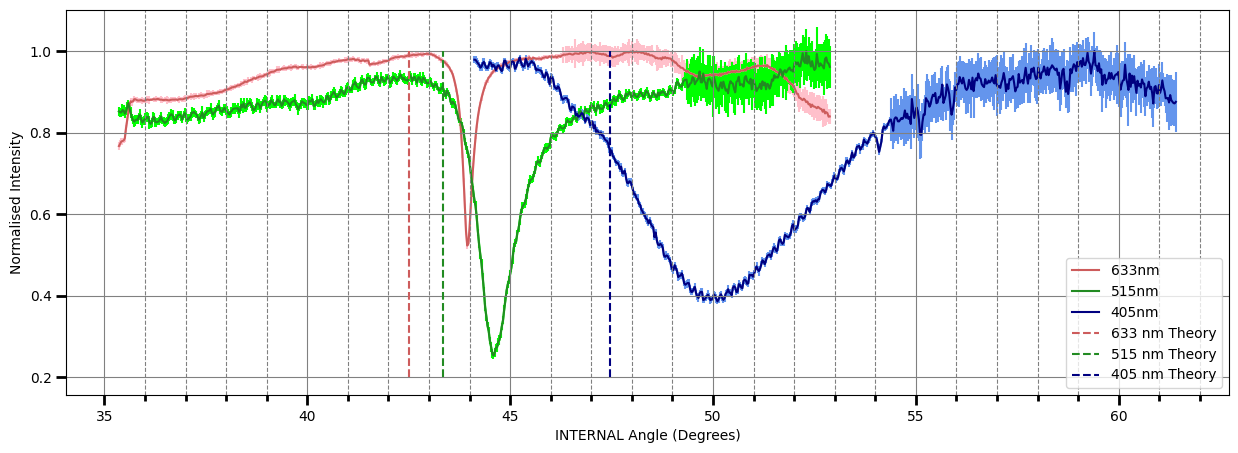
\includegraphics[width=1.5\columnwidth]{wavelengthDependence.png}
				\caption{\label{fig:wavelengthDependence}A plot of all three wavelengths with the $13\,\text{nm}$ prism. The mean voltage is marked by the dark lines and the standard deviation is marked by the lighter region behind them. Note these are strictly errors on the y-axis. Note an uncertainty of approximately 0.5 degrees is present on the x-axis however, this was not included as error-bars in the plot to improve readability}
			\end{figure*}
			
			\begin{table}[]
				\resizebox{\columnwidth}{!}{%
					\begin{tabular}{@{}llll@{}}
						\toprule
						$\lambda$ (nm) & Re($\epsilon_1$) & Theoretical $\theta_\text{int}$ ($^\circ$) & Experimental $\theta_\text{int}$ ($^\circ$) \\ \midrule
						$633$            & $-18.295$          & $42.2$                                       & $43.9 \pm 0.5$                              \\
						$515$            & $-10.687$          & $43.35$                                      & $44.6 \pm 0.5$                              \\
						$405$            & $-4.698$           & $47.45$                                      & $50.0 \pm 0.5$                              \\ \bottomrule
					\end{tabular}%
				}
				\caption{A table of the dielectric constant of silver taken from M. Polyanskiy \cite{refractiveIndex}. Note that the imaginary component of $\epsilon_1$ is neglected as a first approximation.}
				\label{tab:dielectric}
			\end{table}
		
		
		\subsection{Thickness Dependence}
			
			A dependence on the thickness of the silver film is clearly seen throughout the dataset. Figure \ref{fig:thicknessVariation} shows the thickness variation across all three wavelengths. The excitation angle moves towards smaller angles with increasing thickness. An effect of the thickness on the coupling of the waves can be seen in the variation of the depth of the extinction dip, however we don't see a trend across all three wavelengths and no dependence was determined.
			
			\begin{figure}[H]
				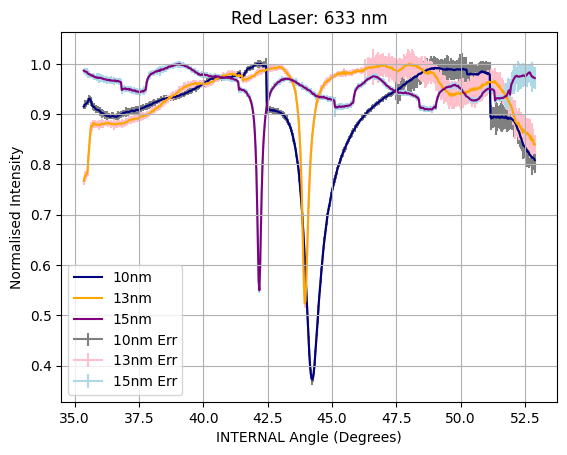
\includegraphics[width=0.75\columnwidth]{redThicknessVariation.png}
				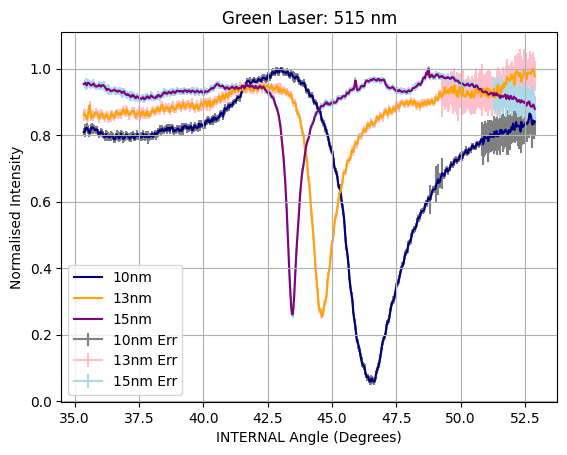
\includegraphics[width=0.75\columnwidth]{greenThicknessVariation.png}
				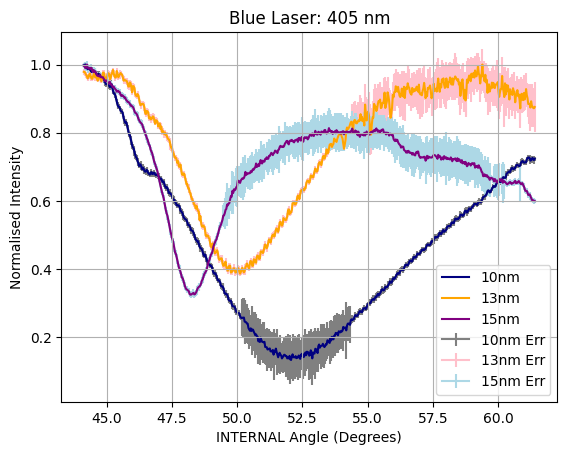
\includegraphics[width=0.75\columnwidth]{blueThicknessVariation.png}
				\caption{\label{fig:thicknessVariation}Plots visualising the variation between each film thickness across all three wavelengths. A thickness dependence of the excitation angle can clearly be visually seen as the minima consistently move towards smaller internal angles as the thickness increases. There appears to be some effect of the film thickness on the coupling as the extent of the extinction varies, however across the dataset no clear correlation can be made.}
			\end{figure}
	
		\subsection{Anomaly found during Red Laser Runs}
			When taking data with the red laser and unexpected result occurred. Large oscillations with a relative intensity amplitude of approximately $0.1$ could be seen in the data, see figure \ref{fig:oscillationsExample}. After attempting to troubleshoot any potential interferences with the data the anomaly seemed unavoidable and a workflow was developed to average multiple data runs together to eliminate the oscillations by destructive interference. This proved to be successful, however while carrying out this workflow after making several consecutive measurements a pattern was apparent from the data. With each consecutive measurement the period of the oscillations was increasing until, after around eight consecutive measurements ($\approx$30 minutes) the period was long enough that the change in intensity was negligible. This change in period is shown in figure \ref{fig:oscillationsExample}. We developed a function to automatically fit a sin wave to each set of data and output its period. An example of this is shown in figure \ref{fig:exampleSin}. Consecutive measurements were made while noting the time that each run started, and using this function a time dependence relation of the period of oscillations was determined. As shown in figure \ref{fig:quadraticDependence} which within the first 22 minutes of laser warm-up the period of these oscillations closely follows a quadratic time dependence. \\
			
			\begin{figure}
				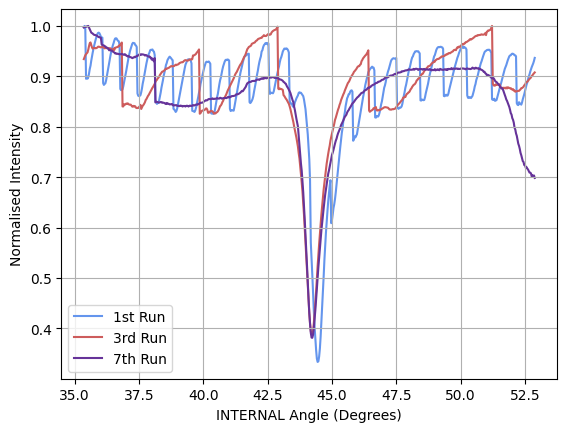
\includegraphics[width=0.85\columnwidth]{oscillationsExample.png}
				\caption{\label{fig:oscillationsExample}An example measurement showing the oscillations apparent in the red laser measurements. Consecutive measurements were taken. This plot displays the 1st, 3rd, and 7th runs showing the apparent change in the oscillations over time. In the 7th run, the oscillations are barely apparent and would not be noticed as such if not for the data taken prior.}
			\end{figure}
		
			\begin{figure}
				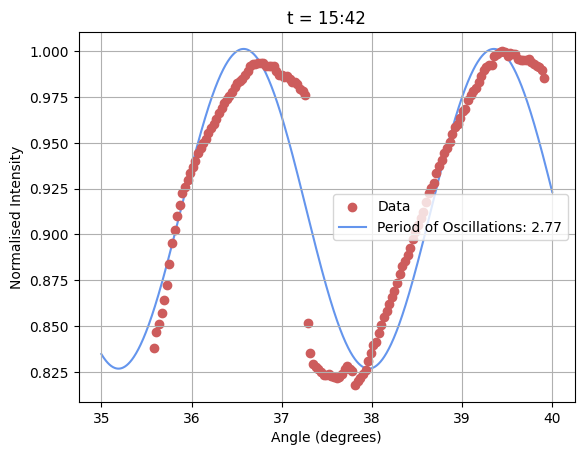
\includegraphics[width=0.85\columnwidth]{exampleTimeDependence.png}
				\caption{\label{fig:exampleSin}An example of how the oscillations in the data closely resemble a sinusoidal wave. This is a sample taken from a standard run of the data collection algorithm approximately 18 minutes after the laser was turned on and started warming up. The period of the sin wave is noted in the legend in degrees.}
			\end{figure}		
		
			\begin{figure}
				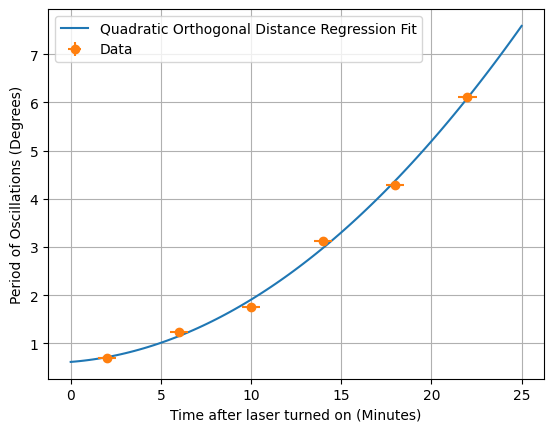
\includegraphics[width=0.85\columnwidth]{quadraticFit.png}
				\caption{\label{fig:quadraticDependence}The quadratic orthogonal distance regression fit of the period of oscillations against the time after the laser was turned on. Following this quadratic curve upwards of thirty seconds the period becomes large enough as to be greater than the range in which the data collection is being carried out.}
			\end{figure}
			
			E. R. Jones describes varying intensity from helium-neon lasers after the light is passed through a linear polariser during an approximately hour long warm-up period after a cold start \cite{jonesPolarisation}. He describes the cause of the effect to be from a few factors: The width of the lasing transition line, the resonant frequencies of the cavity between the mirrors, and the thermal expansion of the laser tube. The figures in this paper and another by Woolsey et al. \cite{woolseyPolarisation} closely match the change in the period of oscillations over time as shown in figure \ref{fig:stillData}. It is important to note that this effect was noticed in the other lasers too but to a much lesser, and in most cases, a negligible effect. This leads us to believe that what was observed is the same effect as demonstrated in the paper by E. R. Jones and that this laser in particular has become somewhat defective with use.
			
			\begin{figure}
				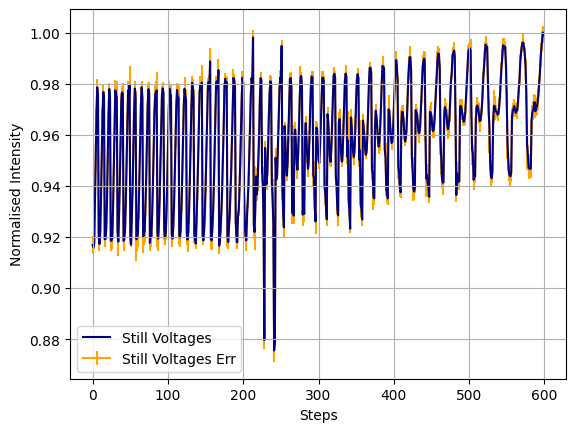
\includegraphics[width=0.85\columnwidth]{stillData.png}
				\caption{\label{fig:stillData}Data taken where the red laser is directly incident on the detector and without the motors turning. The oscillations are still present in this case and can visibly be seen to increase in period over time. Note that although the x axis is represented as steps, these are irrelevant of motor turning and instead mark steps of approximately 0.3 seconds delays between measurements for a full time frame of 3 minutes. The increase in average intensity towards the later part of the plot is unknown but is likely also a part of the "warm-up" process of helium-neon lasers.}
			\end{figure}

	\section{Conclusion}
		
		The aims of this experiment were to determine the excitation angle of surface plasmon resonance (SPR) and observe and investigate the dependencies it has on the wavelength of the incident light and the thickness of the silver film used. We found that the excitation angle of SPR has both an inverse dependence on the wavelength of the incident light and an inverse dependence on the thickness of the silver film.  At a film thickness of 13 nm we determined the excitation angle to be $(43.9\pm0.5)^\circ$, $(44.6\pm0.5)^\circ$, and $(50.0\pm0.5)^\circ$ for the 633 nm, 515 nm, and 405 nm laser respectively. The calculated theoretical angles were outside of the range of uncertainty on these measurements. This is likely due to the approximation of excluding the imaginary component of the dielectric function $\epsilon_1$ and due to not factoring in the thickness of the silver film in the calculation. It was also found that the coupling of the surface plasmon wave with the light was also dependent on the thickness, however more measurements are necessary to determine a trend.
		
		
	\clearpage
	\bibliography{surfacePlasmons}% Produces the bibliography via BibTeX.

		
\end{document}

